\chapter*{Guilin, Xingping et Yangshuo\markboth{Guilin, Xingping et Yangshuo}{}}
\section*{24 octobre 2015}
Je quitte la province du Guizhou pour arriver dans le Guangxi. La route est encore bien défoncée quand j'entends un frottement sur la roue arrière : c'est la jante qui est fissurée. 
\begin{center} 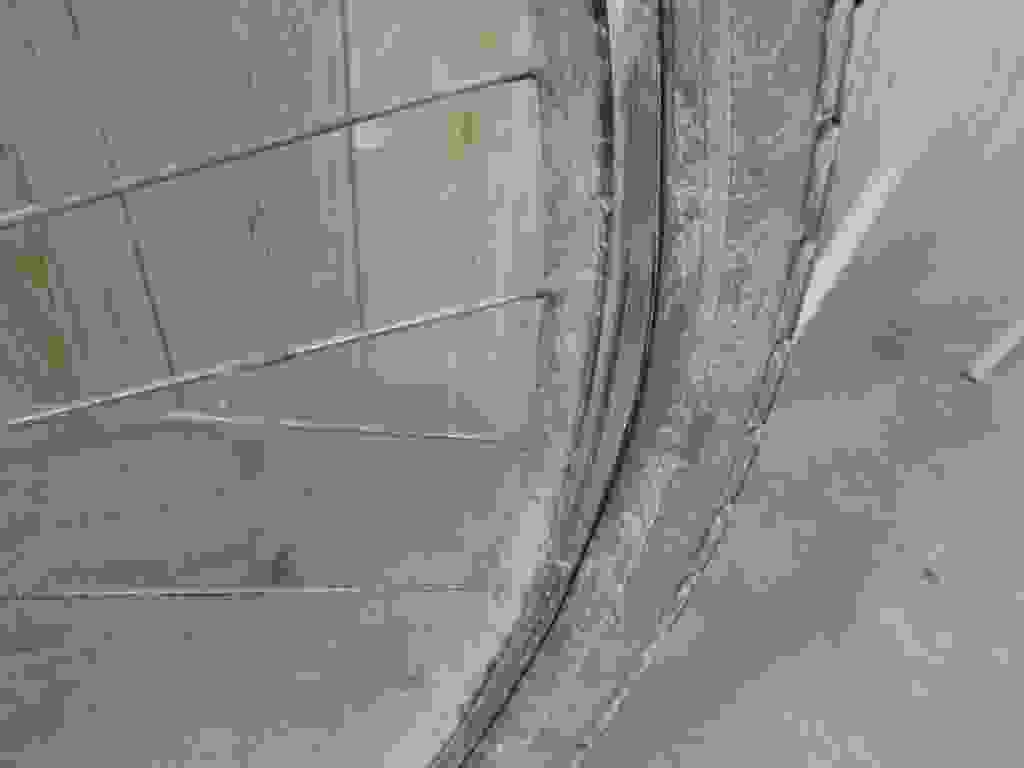
\includegraphics[width=\mywidth]{../wp-content/uploads/2015/10/wpid-oi000027-1024x768.jpg} \end{center}

 Ça tient encore 30km jusqu'à la prochaine ville puis je vais à Guilin en bus pour réparer le vélo. 

\pagebreak

 Guilin sous le soleil. 
\begin{center} 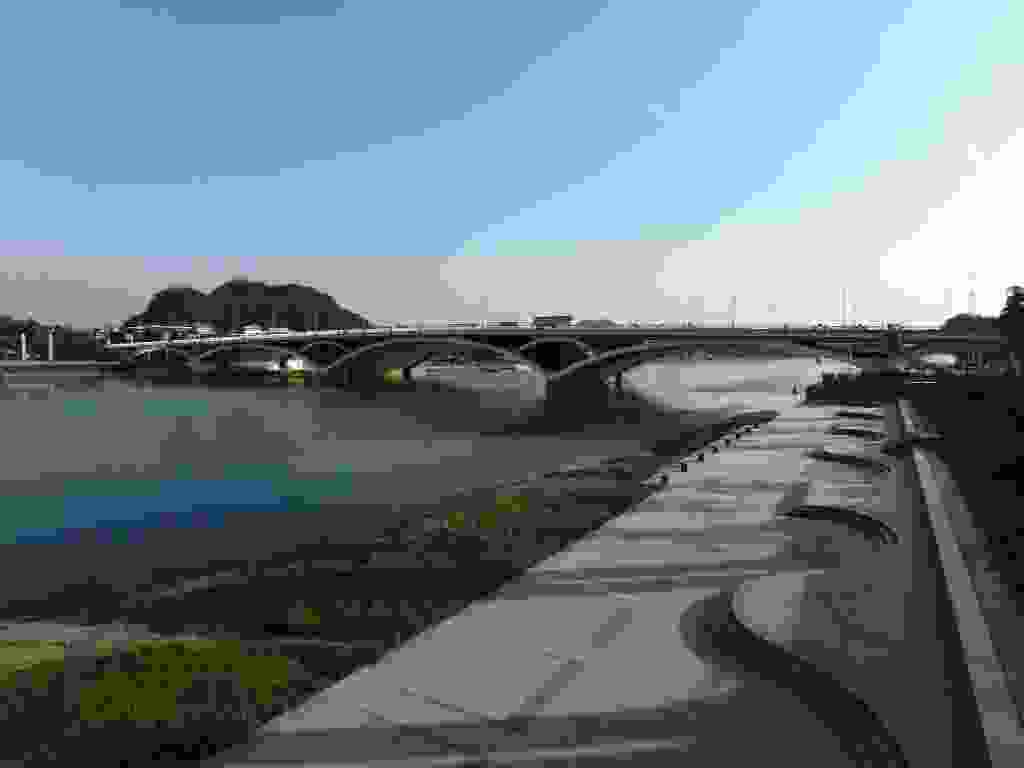
\includegraphics[width=\mywidth]{../wp-content/uploads/2015/10/PA150217-1024x768.jpg} \end{center}
\begin{center} 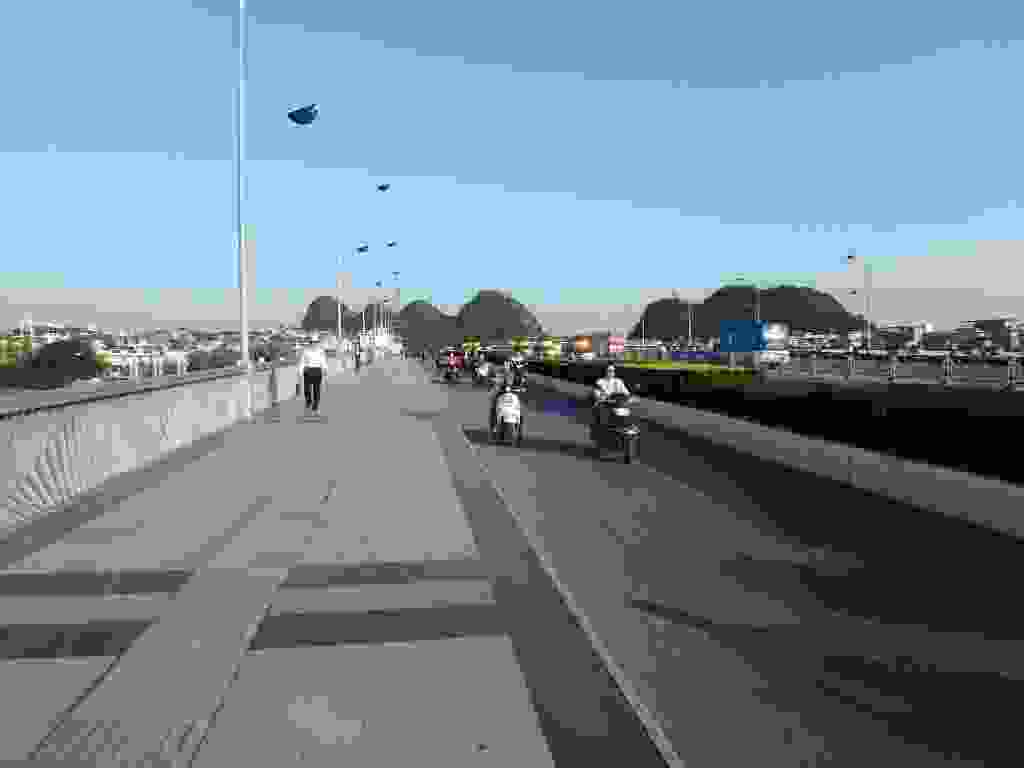
\includegraphics[width=\mywidth]{../wp-content/uploads/2015/10/PA150219-1024x768.jpg} \end{center}
\vspace{-\topsep}
\vspace{-3.25mm}
\pagebreak

~
\begin{center} 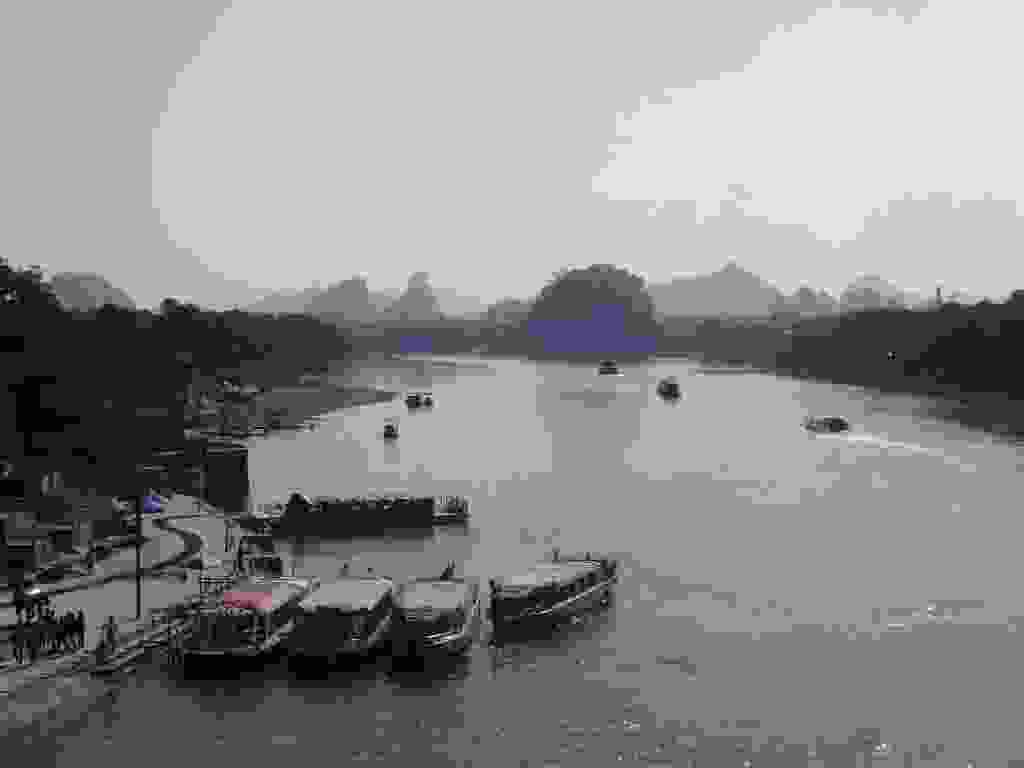
\includegraphics[width=\mywidth]{../wp-content/uploads/2015/10/PA160223-1024x768.jpg} \end{center}
\begin{center} 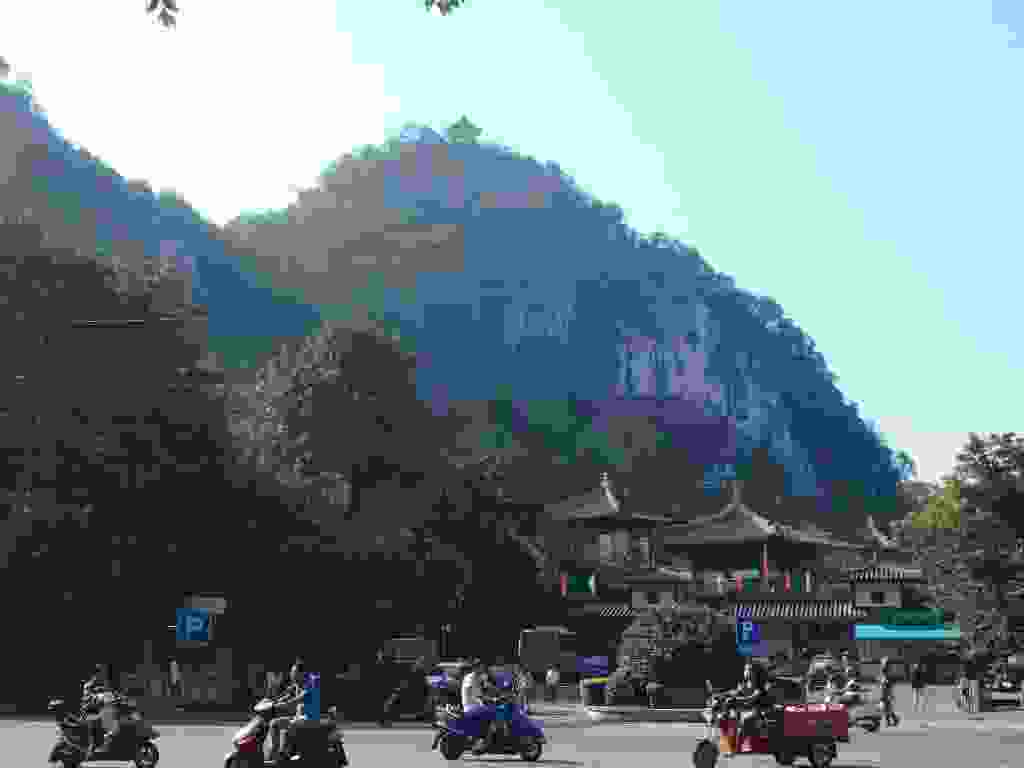
\includegraphics[width=\mywidth]{../wp-content/uploads/2015/10/wpid-oi000028-1024x768.jpg} \end{center}
\vspace{-\topsep}
\vspace{-3.25mm}
\pagebreak

  Pagodes de la Lune et du Soleil. 
\begin{center} 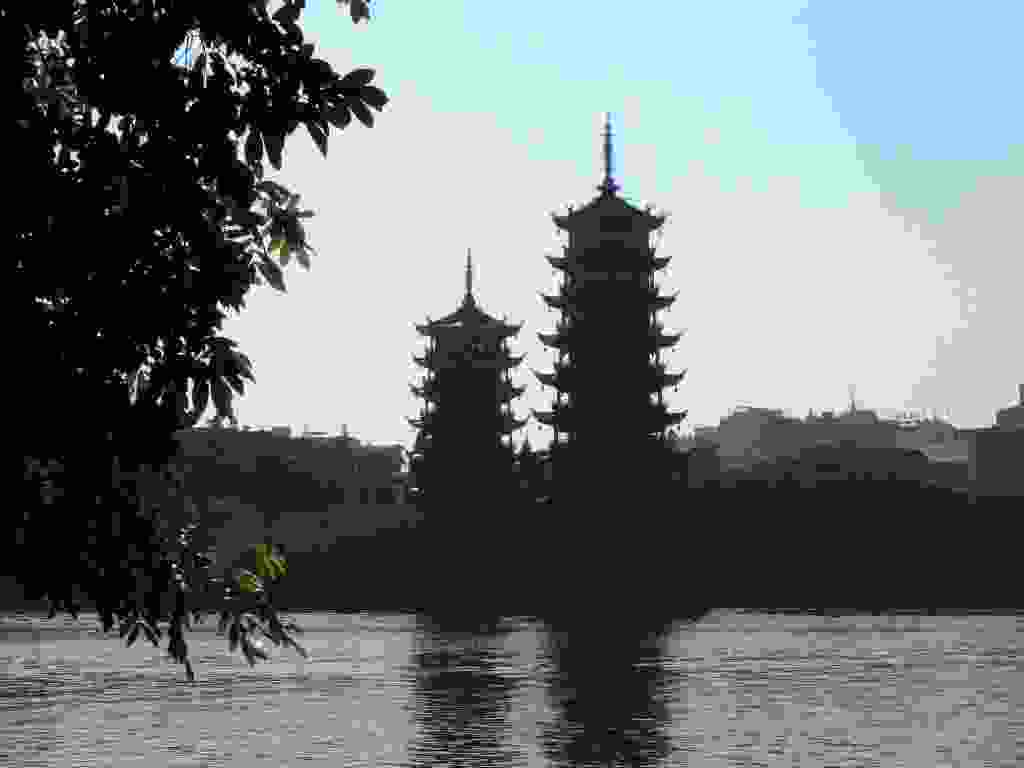
\includegraphics[width=\mywidth]{../wp-content/uploads/2015/10/PA160225-1024x768.jpg} \end{center}

 Joueurs de Majong. \\
\begin{center} 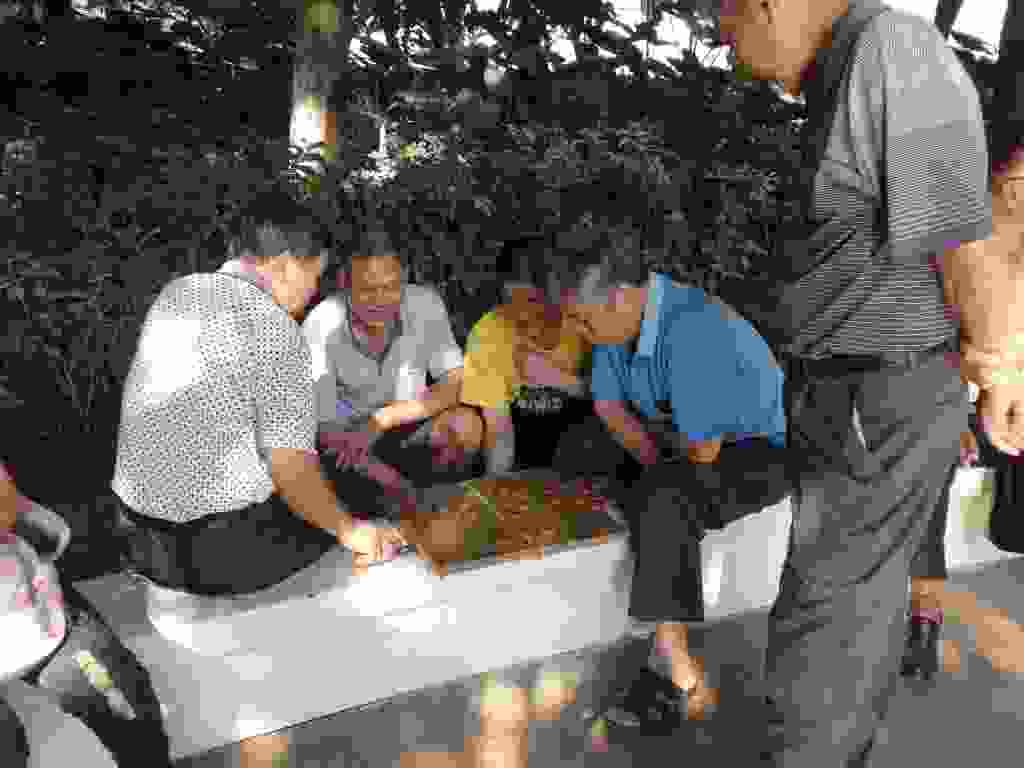
\includegraphics[width=\mywidth]{../wp-content/uploads/2015/10/PA160227-1024x768.jpg} \end{center}
\vspace{-\topsep}
\pagebreak

  Central square. 
\begin{center} 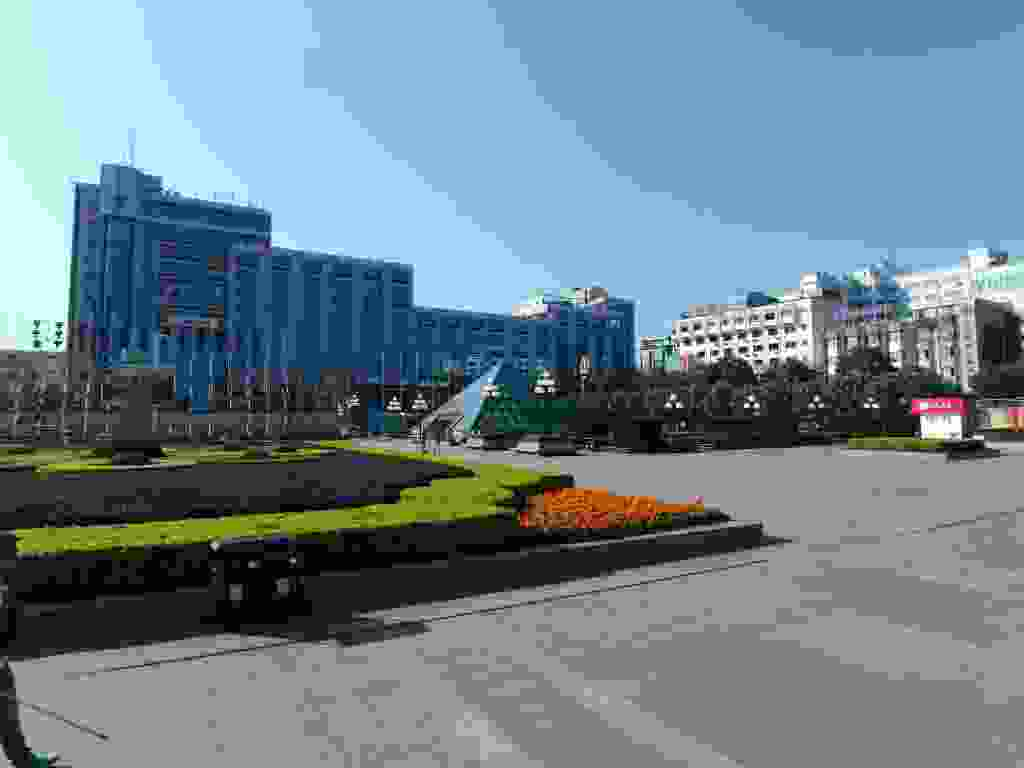
\includegraphics[width=\mywidth]{../wp-content/uploads/2015/10/PA160230-1024x768.jpg} \end{center}

 Une fois la roue arrière changée, je pars vers le sud le long de la rivière Li. 
\begin{center} 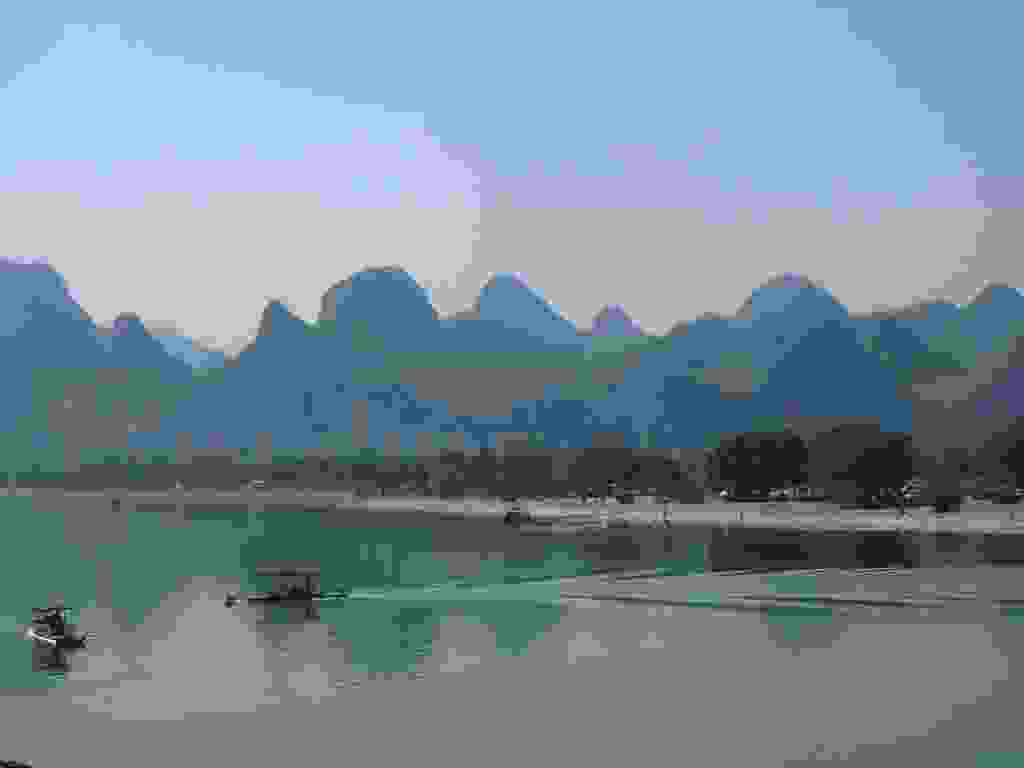
\includegraphics[width=\mywidth]{../wp-content/uploads/2015/10/PA170238-1024x768.jpg} \end{center}
\begin{center} 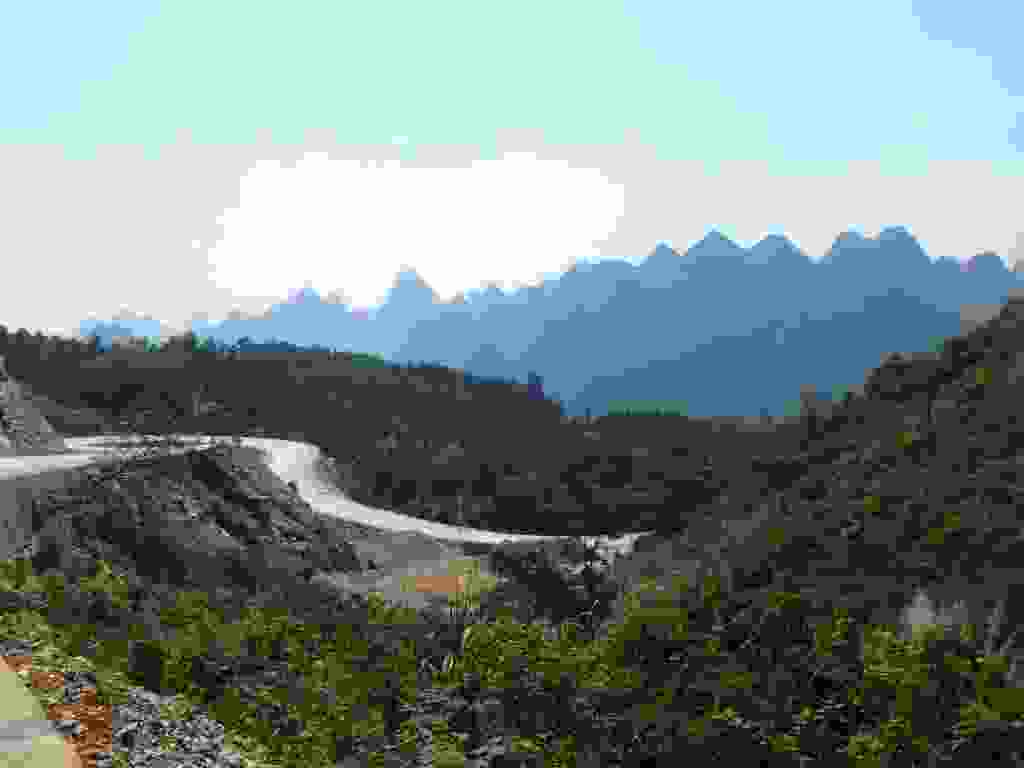
\includegraphics[width=\mywidth]{../wp-content/uploads/2015/10/PA170242-1024x768.jpg} \end{center}
\begin{center} 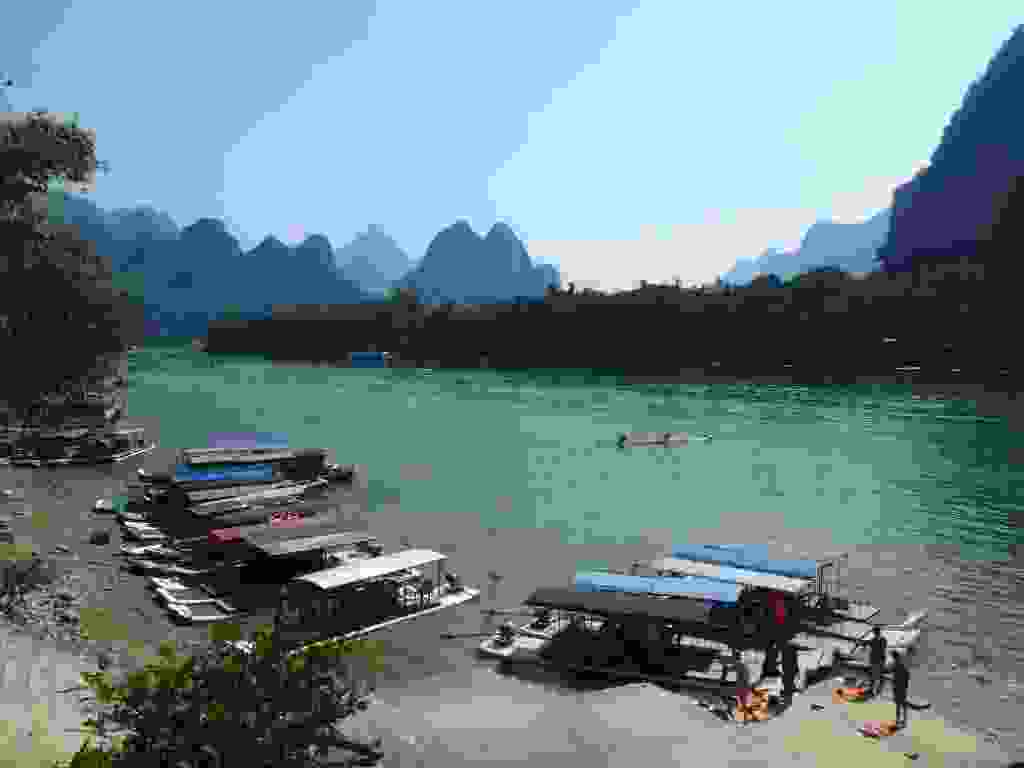
\includegraphics[width=\mywidth]{../wp-content/uploads/2015/10/PA170243-1024x768.jpg} \end{center}
\begin{center} 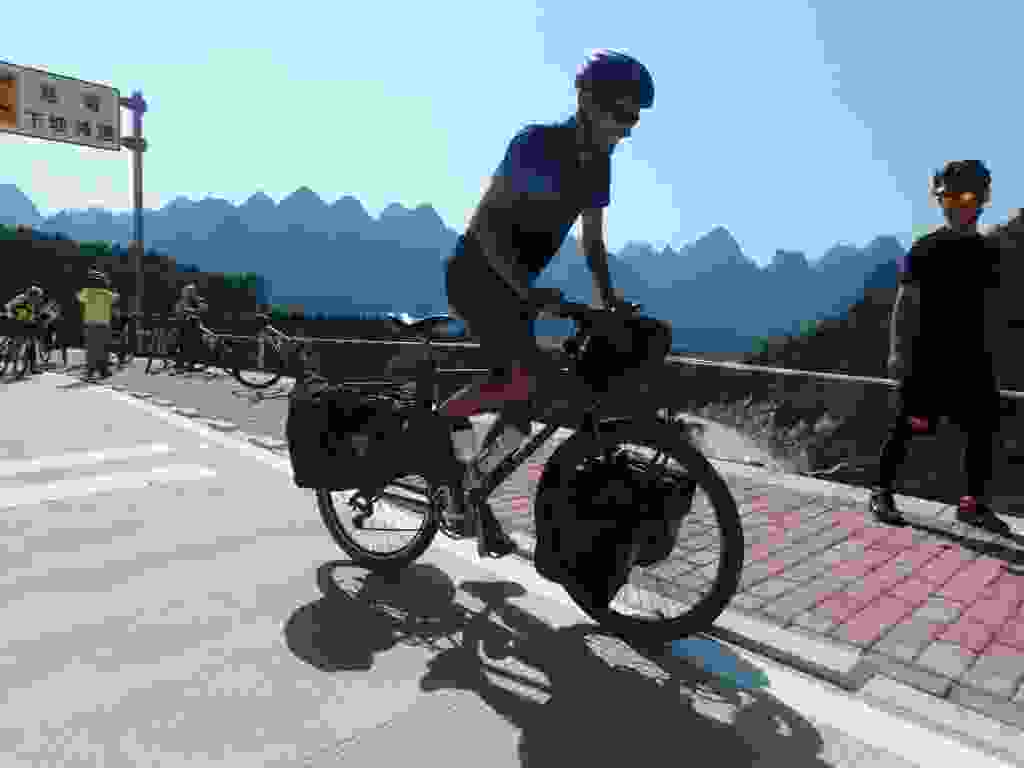
\includegraphics[width=\mywidth]{../wp-content/uploads/2015/10/PA170248-1024x768.jpg} \end{center}

  La route s'élève un peu par endroit.
\begin{center} 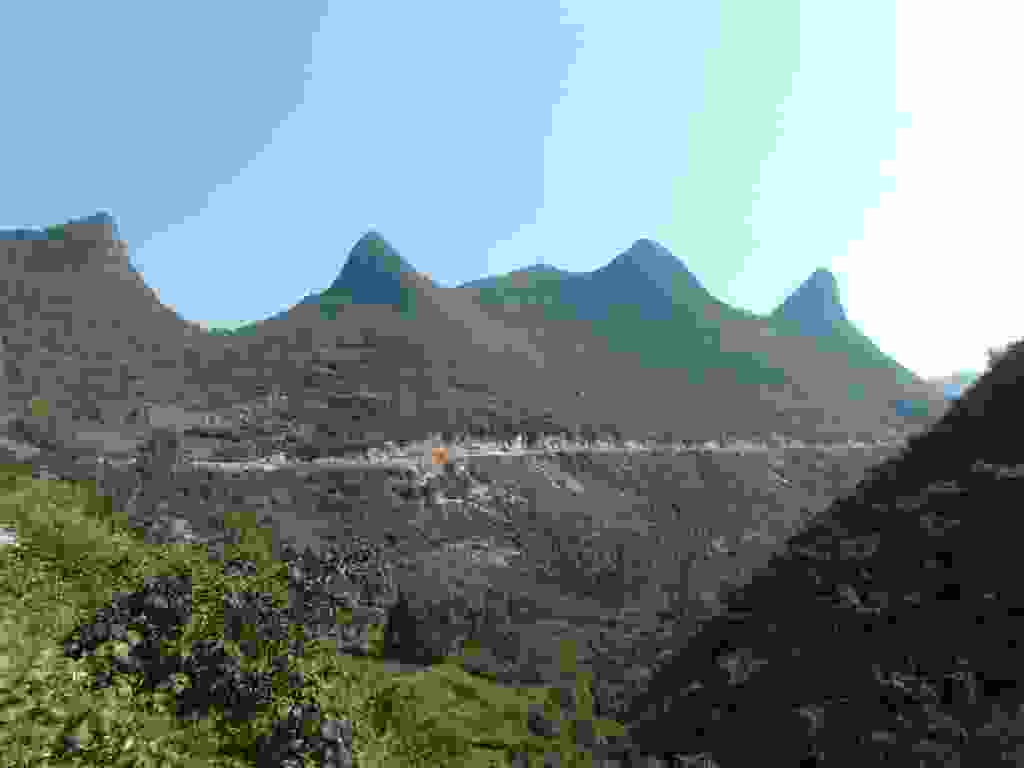
\includegraphics[width=\mywidth]{../wp-content/uploads/2015/10/wpid-oi000030-1024x768.jpg} \end{center}
\begin{center} 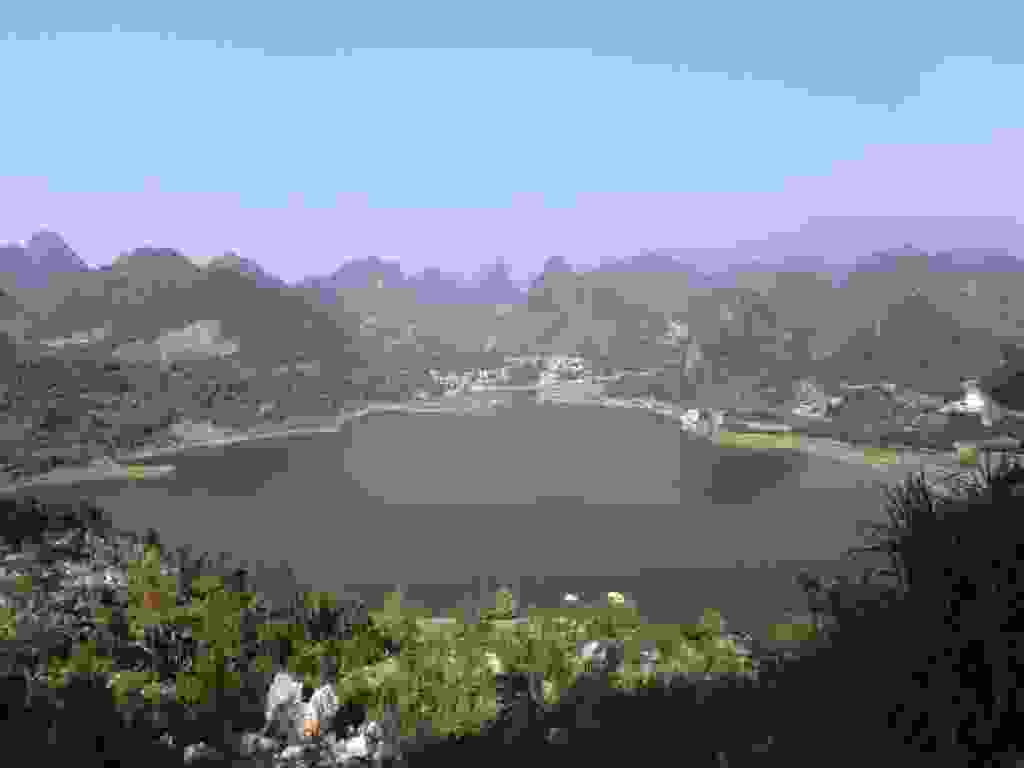
\includegraphics[width=\mywidth]{../wp-content/uploads/2015/10/wpid-oi000032-1024x768.jpg} \end{center}

 Je fais étape à Xingping, village touristique au bord de la rivière. 
\begin{center} 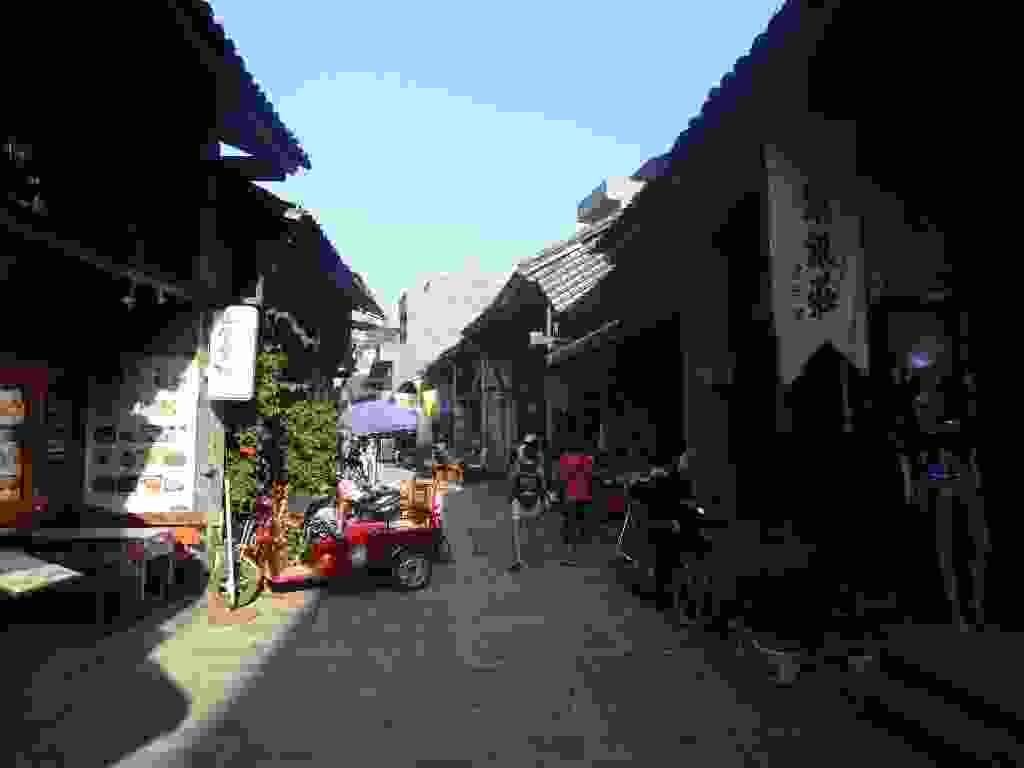
\includegraphics[width=\mywidth]{../wp-content/uploads/2015/10/wpid-oi000033-1024x768.jpg} \end{center}
\begin{center} 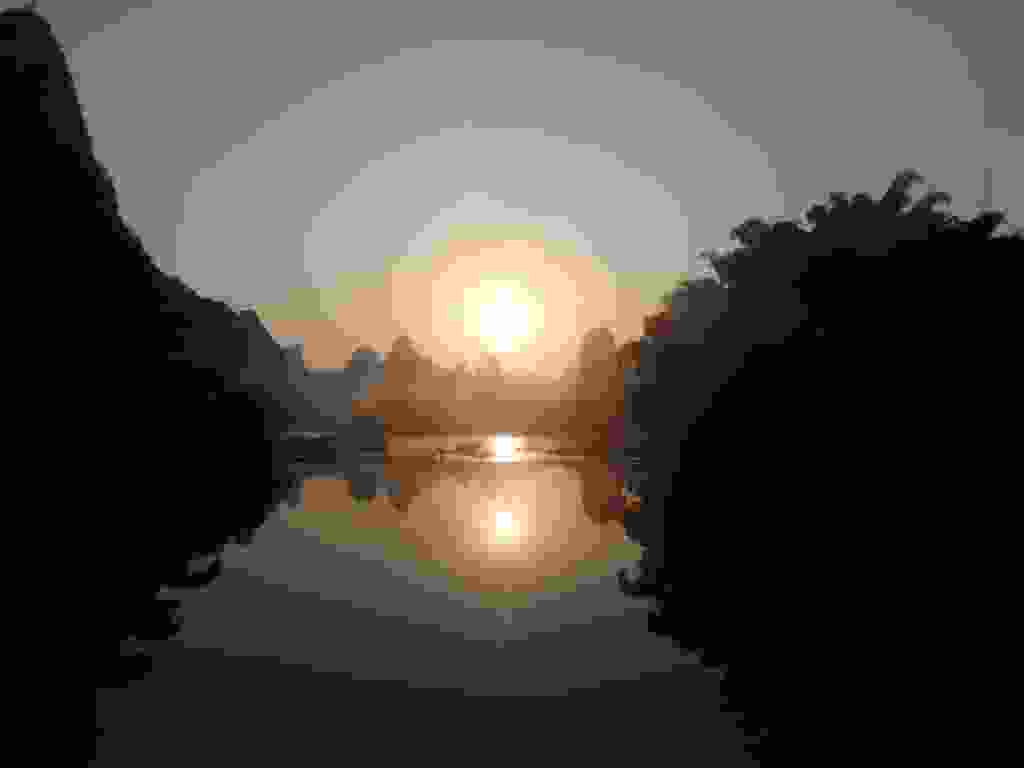
\includegraphics[width=\mywidth]{../wp-content/uploads/2015/10/wpid-oi000034-1024x768.jpg} \end{center}

 Coucher de soleil du haut d'une colline. 
\begin{center} 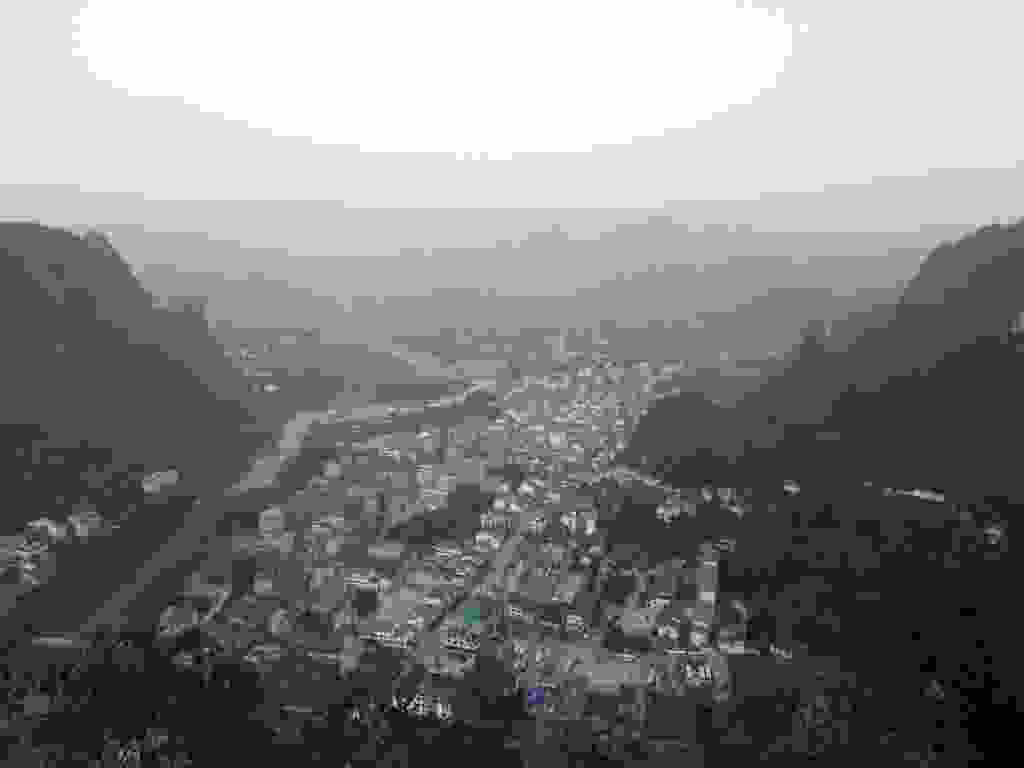
\includegraphics[width=\mywidth]{../wp-content/uploads/2015/10/wpid-oi000035-1024x768.jpg} \end{center}
\begin{center} 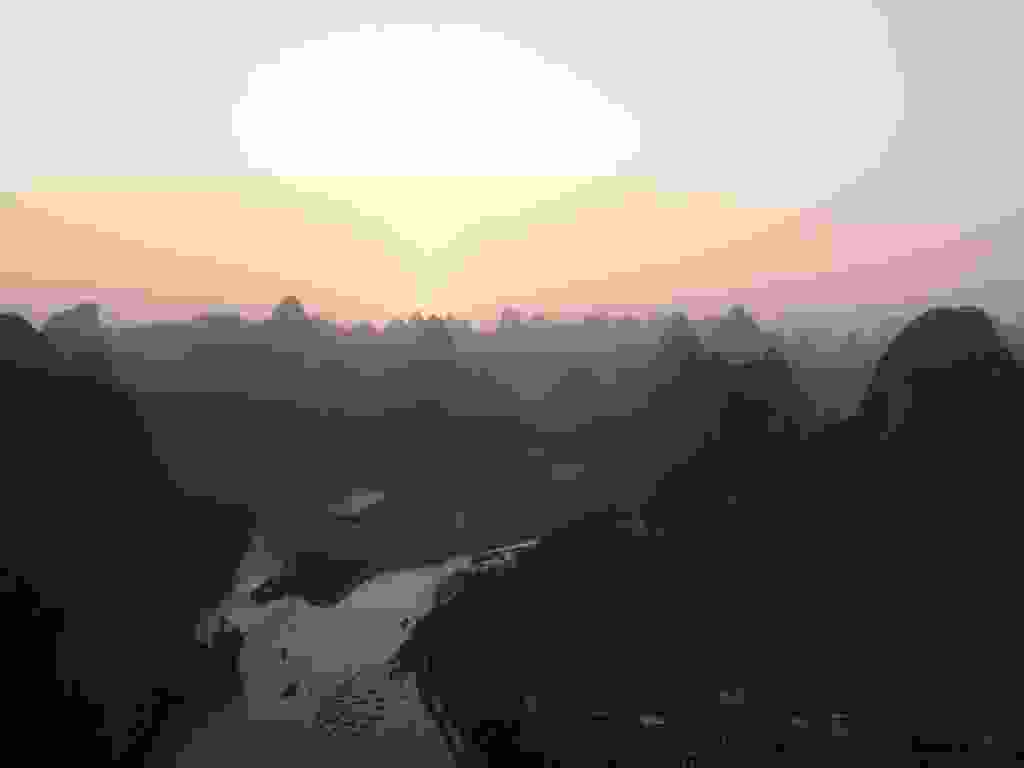
\includegraphics[width=\mywidth]{../wp-content/uploads/2015/10/wpid-oi000036-1024x768.jpg} \end{center}

 Célèbre vue sur la rivière Li. 
\begin{center} 
\includegraphics[width=0.46\textwidth]{../wp-content/uploads/2015/10/wpid-wp-1445656930044.jpg} \end{center}
\begin{center} 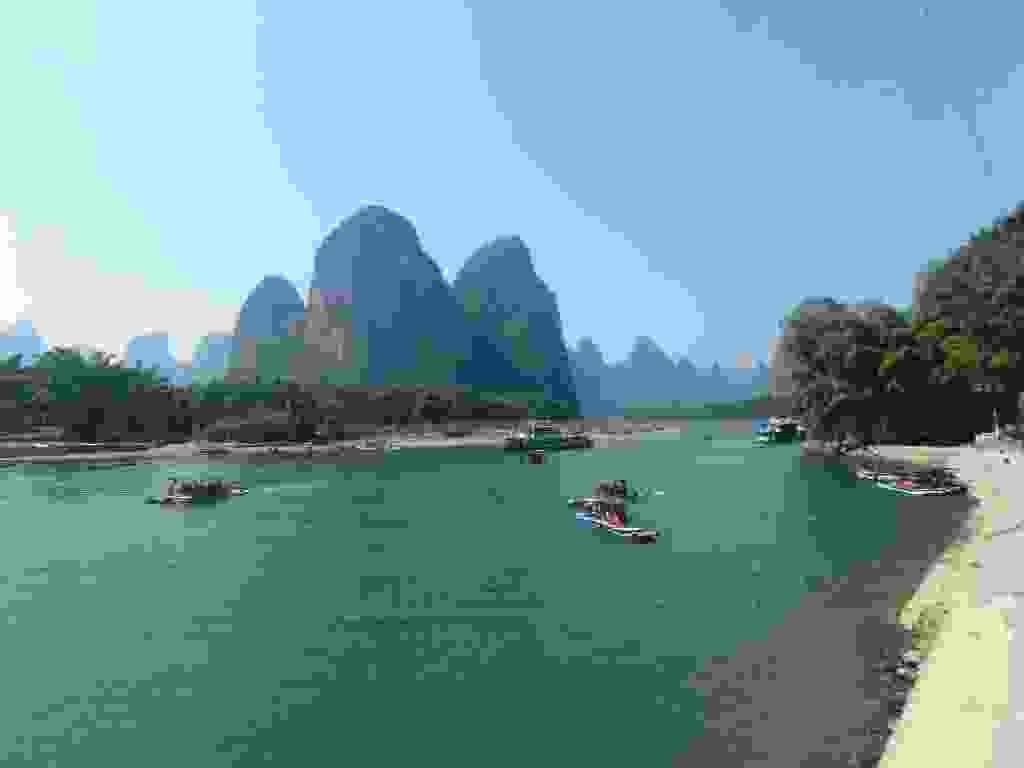
\includegraphics[width=\mywidth]{../wp-content/uploads/2015/10/wpid-oi000037-1024x768.jpg} \end{center}

 Je termine la descente de la rivière à Yangshuo, où je rencontre beaucoup de voyageurs occidentaux : hébergement très bon marché (2.5€ la nuit en dortoir !) et facile pour trouver des pizzas et des burgers. 
\begin{center} 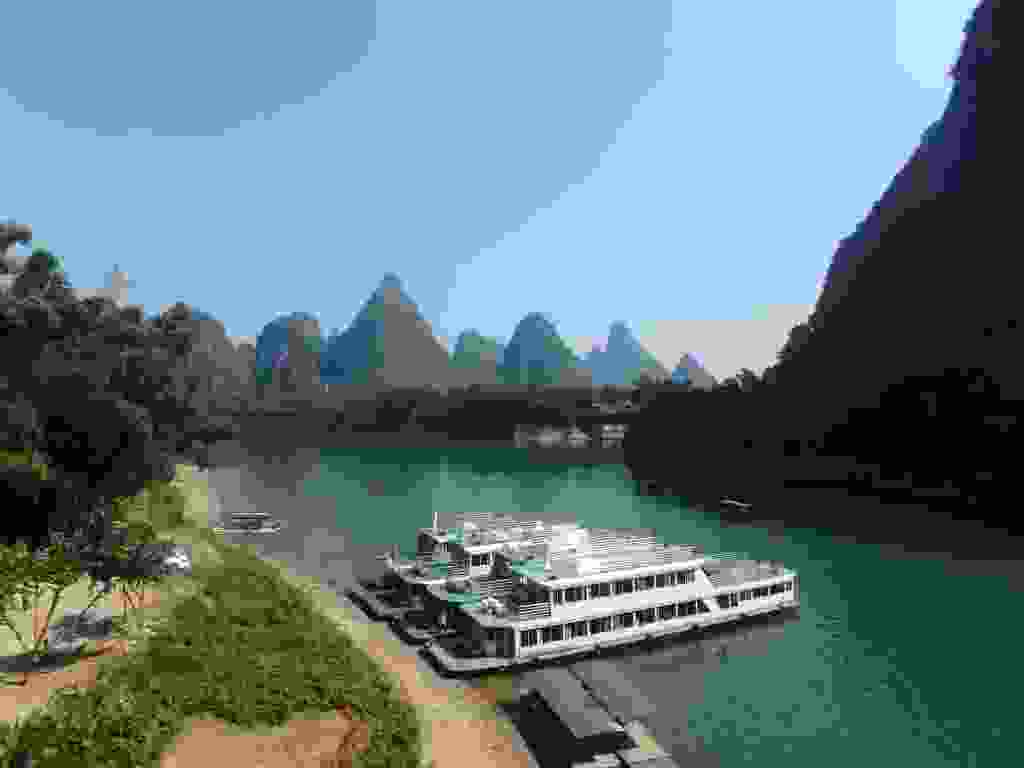
\includegraphics[width=\mywidth]{../wp-content/uploads/2015/10/wpid-oi000039-1024x768.jpg} \end{center}
\begin{center} 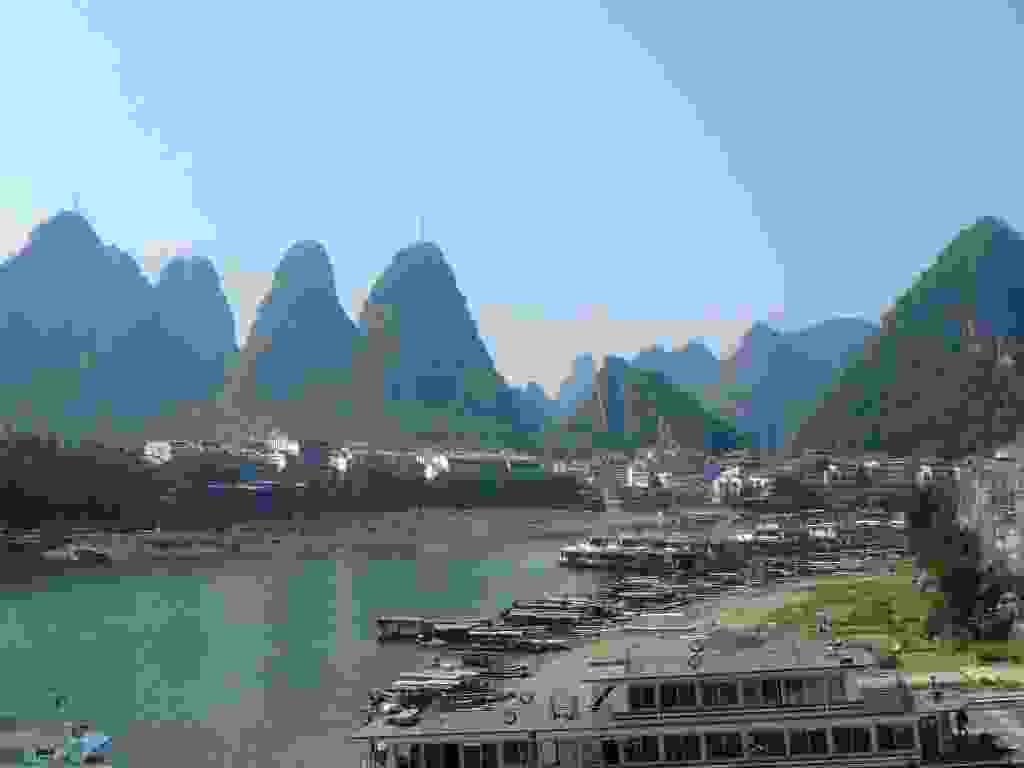
\includegraphics[width=\mywidth]{../wp-content/uploads/2015/10/wpid-oi000038-1024x768.jpg} \end{center}
\begin{center} 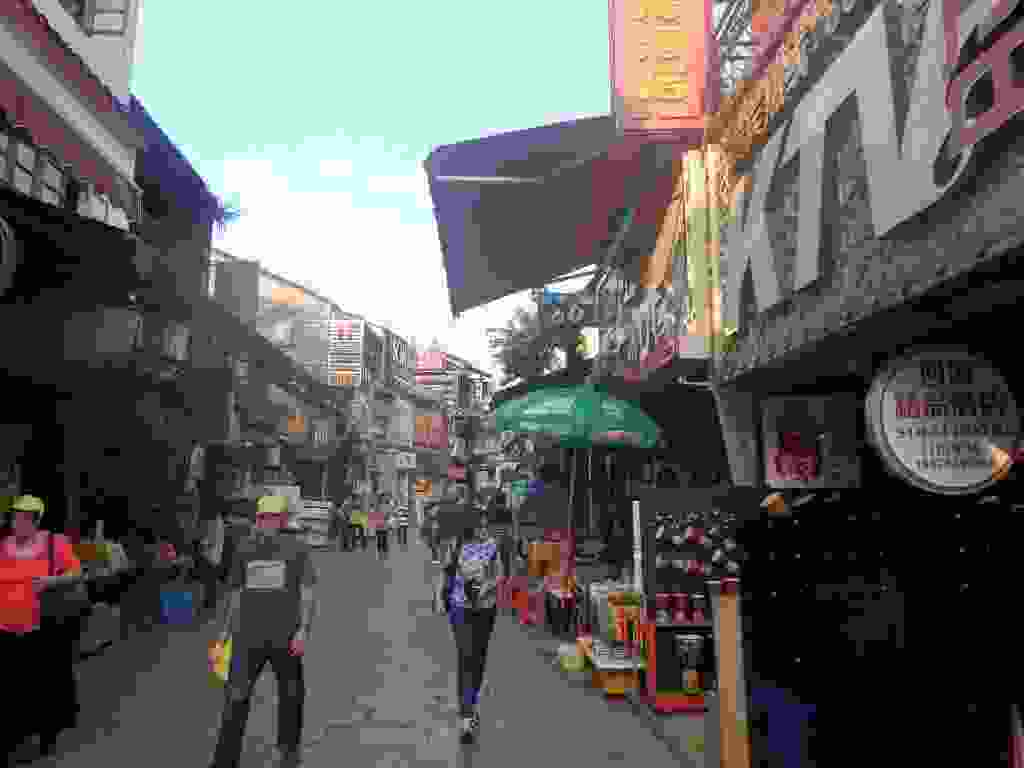
\includegraphics[width=\mywidth]{../wp-content/uploads/2015/10/wpid-oi000040-1024x768.jpg} \end{center}
\begin{center} 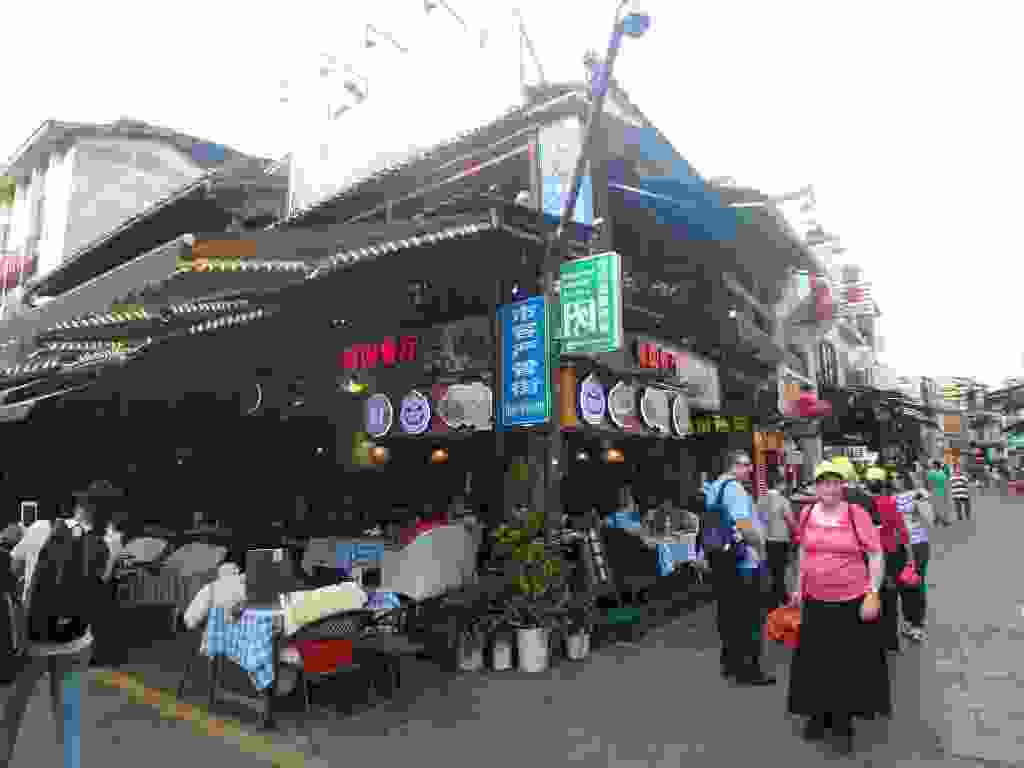
\includegraphics[width=\mywidth]{../wp-content/uploads/2015/10/wpid-oi000041-1024x768.jpg} \end{center}

 C'est la dernière étape en Chine, je prends le bus vers Shenzhen où se trouve la frontière avec Hong Kong.
